\documentclass[crop, tikz]{standalone}
\RequirePackage{luatex85}

\usepackage{fontawesome}
\usepackage{fontspec}
\usepackage{ifthen}
\usetikzlibrary{
    backgrounds,
    patterns,
    mindmap,
    shapes,
    shapes.misc,
    fit,
    trees,
    tikzmark,
    arrows,
    arrows.meta,
    positioning,
    decorations.pathmorphing,
    shapes.geometric,
    decorations.pathreplacing
}

\newfontfamily{\ttfamily}{Fira Code}
\usepackage{fontspec}
\setmainfont{Liberation Sans}
\newfontfamily\ExtraLight{Liberation Sans}
\newfontfamily\Light{Liberation Sans}
\newfontfamily\Book{Liberation Sans}
\newfontfamily\Medium{Liberation Sans}

\definecolor{greenGood}{HTML}{99FF99}
\definecolor{redBad}{HTML}{FF9980}

\makeatletter
\tikzset{btree-key/.style={minimum height=1cm, pattern=north west lines, draw}}
\tikzset{btree-pointer/.style={minimum height=1cm, draw}}
\tikzset{btree-empty/.style={btree-pointer, dashed}}
\tikzset{btree-leaf/.style={fill=greenGood}}
\tikzset{btree-branch/.style={fill=gray!20}}
\tikzset{btree-line/.style={line width=0.5pt}}
\tikzset{btree-path/.style={btree-pointer, minimum width=0.5cm, fill=red, opacity=0.5}}
\tikzset{btree-hide/.style={draw opacity=0, line width=0, pattern=none}}
\tikzset{box/.style={draw, dashed, rounded corners, behind path}}
\tikzset{btree-node/.style={draw, inner sep=0, minimum width=1cm, minimum height=1cm, rounded corners}}
\tikzset{btree-partition1/.style={draw, inner sep=0, minimum width=1cm, minimum height=1cm, rounded corners, fill=red!20}}
\tikzset{btree-partition2/.style={draw, inner sep=0, minimum width=1cm, minimum height=1cm, rounded corners, fill=green!20}}
\tikzset{btree-partition3/.style={draw, inner sep=0, minimum width=1cm, minimum height=1cm, rounded corners, fill=blue!20}}
\tikzset{>=latex}
\tikzset{arrow-pointer/.style={
        single arrow,
        minimum height=1.5cm,
        inner sep=3pt,
        line width=1pt,
        draw,
        color=gray,
        single arrow tip angle=45,
        single arrow head extend=0.1cm
    }
}

\newcommand{\btreenode}[5] {
    \path
      node[btree-pointer, #2, #3] (pointer1#1) {}
      node[btree-key, right=0 of pointer1#1, #3] (sep1#1) {}
      node[btree-key, left=0 of pointer1#1, #3] (sep2#1) {}
      node[btree-pointer, right=0 of sep1#1, #3] (pointer2#1) {}
      node[btree-pointer, left=0 of sep2#1, #3] (pointer3#1) {}
      node[btree-key, right=0 of pointer2#1, #3] (sep3#1) {}
      node[btree-key, left=0 of pointer3#1, #3] (sep4#1) {}
      node[draw, inner sep=0, behind path, #4,
          fit=(pointer1#1)(pointer2#1)(pointer3#1)
              (sep1#1)(sep2#1)(sep3#1)(sep4#1)
      ] (node#1) {};

      \ifthenelse{ \equal{#5}{show-pointers} } {
            \coordinate[below=0.5 of pointer1#1] (heap-pointer1#1);
            \coordinate[below=0.5 of pointer2#1] (heap-pointer2#1);
            \coordinate[below=0.5 of pointer3#1] (heap-pointer3#1);

            \draw[->, btree-line] (pointer1#1.south) -- (heap-pointer1#1.north);
            \draw[->, btree-line] (pointer2#1.south) -- (heap-pointer2#1.north);
            \draw[->, btree-line] (pointer3#1.south) -- (heap-pointer3#1.north);
      } {}
}

\makeatother

\begin{document}
    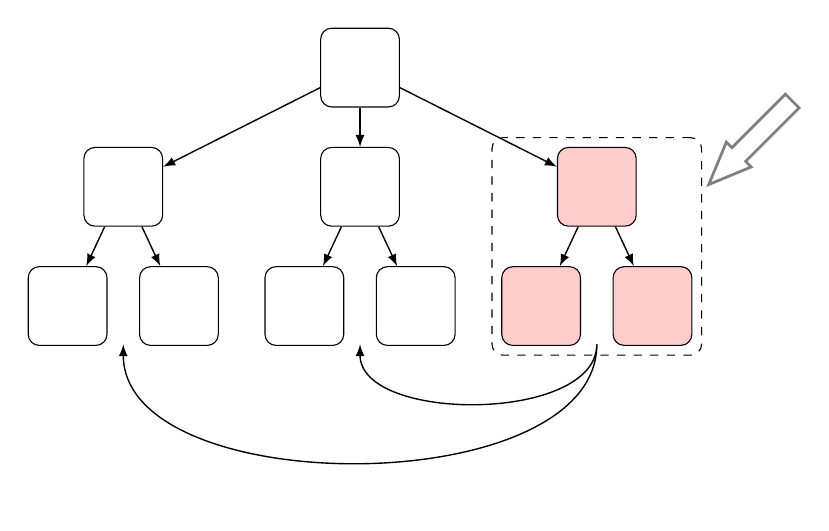
\begin{tikzpicture}[]
        \node[btree-node] (node1) {};

        \node[btree-node, below=0.5cm of node1.south west, xshift=-2.5cm] (node2) {};
        \node[btree-node, below=0.5cm of node1.south] (node3) {};
        \node[btree-partition1, below=0.5cm of node1.south east, xshift=2.5cm] (node4) {};

        \node[btree-node, below=0.5cm of node2.south west, xshift=-0.2cm] (node5) {};
        \node[btree-node, below=0.5cm of node2.south east, xshift=0.2cm] (node6) {};

        \node[btree-node, below=0.5cm of node3.south west, xshift=-0.2cm] (node7) {};
        \node[btree-node, below=0.5cm of node3.south east, xshift=0.2cm] (node8) {};

        \node[btree-partition1, below=0.5cm of node4.south west, xshift=-0.2cm] (node9) {};
        \node[btree-partition1, below=0.5cm of node4.south east, xshift=0.2cm] (node10) {};

        \draw[->, btree-line] (node1) -- (node2);
        \draw[->, btree-line] (node1) -- (node3);
        \draw[->, btree-line] (node1) -- (node4);

        \draw[->, btree-line] (node2) -- (node5);
        \draw[->, btree-line] (node2) -- (node6);

        \draw[->, btree-line] (node3) -- (node7);
        \draw[->, btree-line] (node3) -- (node8);

        \draw[->, btree-line] (node4) -- (node9);
        \draw[->, btree-line] (node4) -- (node10);

        \node[arrow-pointer, right=2cm of node9.center, rotate=-135, xshift=-2.7cm, yshift=-1cm] {};
        \node[box, fit=(node4)(node9)(node10)] {};
        \node[below=3cm of node3.center, minimum height=1cm] {};

        \draw[->, btree-line] ([yshift=-2cm]node4.center)
            .. controls ([yshift=-3cm] node4) and ([yshift=-3cm] node3) ..
            ([yshift=-2cm]node3.center);
        \draw[->, btree-line] ([yshift=-2cm]node4.center)
            .. controls ([yshift=-4cm] node4) and ([yshift=-4cm] node2) ..
            ([yshift=-2cm]node2.center);

    \end{tikzpicture}
\end{document}
